\documentclass[11pt]{article}

% required libs
%\usepackage[margin=0.75in]{geometry}
\usepackage{amsmath}
\usepackage{tikz}

%tikz config
\usetikzlibrary{arrows.meta,calc,positioning,decorations.markings}
\pagestyle{empty}
\definecolor{flatblue}{RGB}{31,110,165}
\definecolor{curvedred}{RGB}{184,71,65}
\definecolor{lightgray}{RGB}{150,158,166}
\tikzset{
 particle/.style={circle,fill=black,inner sep=1.55pt},
 centerparticle/.style={circle,fill=white,draw=black,thick,inner sep=2.3pt},
 fieldarrow/.style={-{Stealth[length=2.2mm]},line width=0.75pt},
 laserbeam/.style={line width=1.6pt,flatblue},
 armbeam/.style={line width=1.6pt,curvedred},
 mirror/.style={line width=2.4pt,black},
}

\usepackage[T1]{fontenc}
\usepackage[utf8]{inputenc}

\usepackage{amsmath, amssymb, amsfonts}
\usepackage{mathtools}
\usepackage{physics}

\usepackage{graphicx}
\usepackage{hyperref}

\graphicspath{{../figures}}
%\newcommand{\dd}{\,\mathrm{d}}
\newcommand{\e}{\mathrm{e}}
\newcommand{\ii}{\mathrm{i}}

\title{Problem 2: Acceleration versus Curavture}
\author{Ethan Harriman \\ email: elhphysics1299@gmail.com \\ GitHub: https://github.com/Eharriman \\ Website: https://elhphysics.substack.com}
\date{\today}

\begin{document}
\maketitle

\section{Problem}

\textit{A Uniform Gravitational Field} Calculate the Riemann curvature for the metric

\begin{equation}
    \label{uniform metric}
    ds^2 = -(1 + gx)^2 dt^2 + dx^2 + dy^2 + dz^2
\end{equation}

thereby showing this spacetime is flat. Find a coordinate transformation that puts this metric into the usual Minkowski form.

\subsection{Introduction}

This is a seemingly inncocuous problem in Hartle's introductory text on General Relativity. It permits a learner to practice calculating the Riemann curvature components from hand; and further induces the reader to consider the meaning of said calculations. But in solving, and further reflecting on this problem, one can achieve significant intuition and understanding into the nature of space, time, and the meaning of realtivity.

The problem itself is straightforward: given metric \eqref{uniform metric}, calculate the Riemann curvature compoents $R^{\alpha} _{\beta \gamma \delta}$. A flat spacetime is one whose Riemann components vanish (in all coordinates), and thus we aim to demonstrate that:

\begin{equation}
    \label{flat Riemann}
    R^{\alpha} _{\beta \gamma \delta} = 0.
\end{equation}

Further, we will attempt to produce a coordinate transformation, $x \rightarrow x'$, that reduces the metric \eqref{uniform metric} to a Minkowski flat spacetime form. Explicitly:

\begin{equation}
    \label{minkowski metric}
    ds^2 = -dt'^2 + dx'^2 + dy'^2 + dz'^2.
\end{equation}

These two results would demonstrate the following physical facts: 1) the spacetime described by the metric \eqref{uniform metric} is flat, even though on first glance it does not look so; 2) there exists a coordinate transformation under which the spacetime is described by the usual flat Minkowski metric. Prior to solving the above-stated problem, a thought-experiment is worthwhile to encourage the specific line of inquiry this article will tackle.

\subsection{Acceleration or Gravity?}

When I was first introduced to General Relativity, a specific, all-too-familiar, heuristic was used to motivate the intuition behind the so-called Equivalence Principle. 

Consider an observer in an elevator whose construction is sufficient to isolate the observer from any external signals/light/etc. The observer has some basic physical devices with which they can conduct rudimentary physics experiments. External agents have set up, for the internal observer, one of two possible physical scenarios: 1) the elevator is stationary on the surface of a planet which has a static uniform gravitational field whose acceleration is $g=9.8 \mathrm{m}/\mathrm{s}^2$; Or 2) the elevator is pulled by an accelerating spaceship through empty space at a constant, uniform, acceleration of $9.8 \mathrm{m}/\mathrm{s}^2$.

Question: are there any experiments the internal observer can perform that would allow them to discriminate between the physical scenario a) and b)? In other words, are there any experiments that the internal observer could perform that would allow them to determine whether they were under a uniform gravitational field, or under uniform accelerated motion?

Those familiar with descriptions of the Equivalence Principle would answer in the negative. All \textit{local} experiments will be indinguishable between scenario a) and b). Objects dropped will accelerate down to the floor with the same rates. In the former scenario this is due to the uniform gravitational acceleration, in the latter case this is due to Newton's First Law: the elevator floor accelerates up to the released object at the same acceleration as the uniform gravitiational field. The Equivalence Principle seems to indicate that these two scenarios are identical. I recall learning that the beauty of General Relativity was Einstein's insight: if these two scenarios are indistinguishable, then their physical origin should be indistinguishable as well. That is: acceleration and gravity are one in the same.

\section{Vanishing Curvature}

\subsection{Specific Case}

Consider the formula for the Christoffel symbols

\begin{equation}
    \label{christ-awful-1}
    \Gamma^{\alpha}_{\beta \gamma} = \frac{1}{2} g^{\alpha \delta} \left( \partial_{\gamma} g_{\delta \beta} + \partial_{\beta} g_{\delta \gamma} - \partial_{\delta} g_{\beta \gamma}\right)
\end{equation}

where we use the shorthand $\partial_{\gamma} = \frac{\partial}{\partial x^{\gamma}}$. Metric \eqref{uniform metric} is diagonal and thus fixes the condition $\alpha = \delta$. The only valid choices are $\alpha = t, x$, as the other components result in vanishing first derivatives. Consider the case $\alpha = t$


\begin{equation}
    \label{christ-awful-t}
    \Gamma^{t}_{\beta \gamma} = \frac{1}{2} g^{t t} \left( \partial_{\gamma} g_{t t} + \partial_{t} g_{t t} - \partial_{t} g_{\beta \gamma}\right).
\end{equation}

For the uniform metric the time derivatives vanish. The only non-vanishing component is found with $\gamma = x$

\begin{equation}
    \label{christ-awful-t-2}
    \Gamma^{t}_{t x} = \frac{1}{2} g^{t t} \left( \partial_{x} g_{t t}\right).
\end{equation}

$g^{t t}$ can be found using the identity

\begin{equation}
    \label{metric-kronecker}
    g^{\alpha \beta} g_{\alpha \beta} = \delta^{\alpha} _{\beta}.
\end{equation}

And the derivative in \eqref{christ-awful-t-2} is

\begin{equation}
    \label{x-derivative-explicit}
    \partial_{x} g_{t t} = 2 (1 + gx) g.
\end{equation}

Thus

\begin{equation}
    \label{christ-awful-t-3}
    \Gamma^{t}_{t x} = g (1 + gx)^{-1}.
\end{equation}

Using the symmetry of the Christoffel symbols we also have $\Gamma^{t}_{t x} = \Gamma^{t}_{x t}$. The other case is determined with $\alpha = x$. This results in

\begin{equation}
    \label{christ-awful-x}
    \Gamma^{x}_{t t} = \frac{1}{2} g^{x x} \left( \partial_{t} g_{\delta t} + \partial_{t} g_{\delta t} - \partial_{\delta} g_{t t}\right).
\end{equation}

Using the same arguments as above, this results in

\begin{equation}
    \label{christ-awful-x-1}
    \Gamma^{x}_{t t} = \frac{1}{2} g^{x x} \left( - \partial_{x} g_{t t}\right) = g(1 + gx).
\end{equation}

In coordinate components the Riemann curvature is

\begin{equation}
    \label{Riemmann-curv-formula}
    R^{\alpha} _{\beta \gamma \delta} = \partial_{\gamma} \Gamma^{\alpha}_{\beta \delta} - \partial_{\delta} \Gamma^{\alpha}_{\beta \gamma} + \Gamma^{\alpha}_{\gamma \epsilon} \Gamma^{\epsilon}_{\beta \delta} - \Gamma^{\alpha}_{\delta \epsilon} \Gamma^{\epsilon}_{\beta \gamma}.
\end{equation}

Fix the only case with non-zero Christoffel symbols using $\alpha = t$

\begin{equation}
    \label{Riemmann-curv-formula-t-x}
    R^{t} _{\beta \gamma \delta} = \partial_{\gamma} \Gamma^{t}_{\beta \delta} - \partial_{\delta} \Gamma^{t}_{\beta \gamma} + \Gamma^{t}_{\gamma \epsilon} \Gamma^{\epsilon}_{\beta \delta} - \Gamma^{t}_{\delta \epsilon} \Gamma^{\epsilon}_{\beta \gamma}.
\end{equation}

With only three non-vanishing Christoffel symbols (two of which are identical by symmetry) we have only two cases. Consider $\beta = t$ and $\delta = x$. The only non-zero derivative forces $\gamma = x$. Thus:

\begin{equation}
    \label{Riemmann-curv-formula-t-x}
    R^{t} _{t x x} = \partial_{x} \Gamma^{t}_{t x} - \partial_{x} \Gamma^{t}_{t x} + \Gamma^{t}_{x \epsilon} \Gamma^{\epsilon}_{t x} - \Gamma^{t}_{x \epsilon} \Gamma^{\epsilon}_{t x}.
\end{equation}

The only non-vanishing Christoffel symbol forces $\epsilon = t$. The double Christoffel terms thus vanish by symmetry. So too does the first derivatives. Thus

\begin{equation}
    \label{Riemmann-curv-formula-t-x-2}
    R^{t} _{t x x} = 0.
\end{equation}

An identical argument with $\alpha = x$ shows that all Riemann components vanish. Recall that the Riemann curvature tensor is used to quantify local curvature. If all components vanish then the space is flat. We thus conclude that the spacetime described by \eqref{uniform metric} is flat.

\subsection{The General Uniform Metric}

It is worth proving that \eqref{uniform metric} is an example of a more general case. Consider a metric of the form

\begin{equation}
    \label{gen-uni-metric}
    ds^2  = -f^2(x) dt^2 + dx^2 + dy^2 + dz^2,
\end{equation}

where $f(x)$ is a function of the coordinate x alone. The Christoffel symbols for this metric reduce to two cases. Firstly

\begin{equation}
    \label{christ-awful-t-f}
    \Gamma^{t}_{\beta \gamma} = \frac{1}{2} g^{t t} \left( \partial_{\gamma} g_{t t} + \partial_{t} g_{t t} - \partial_{t} g_{\beta \gamma}\right).
\end{equation}

This simplifies with the only non-zero derivative setting $\gamma = x$

\begin{equation}
    \label{christ-awful-t-f2}
    \begin{split}
    \Gamma^{t}_{t x} & = \frac{1}{2} g^{t t} \left( \partial_{x} g_{t t}\right) \\
    & = \frac{1}{2} (-f^{-2}(x)) \partial_{x} (f^2(x)) \\
    & = f^{-2}(x) f(x) f'(x) \\
    & = \frac{f'(x)}{f(x)} = \Gamma^{t}_{x t}.
    \end{split}
\end{equation}

The second case has $\alpha = x$

\begin{equation}
    \label{christ-awful-x-f}
    \Gamma^{x}_{\beta \gamma} = \frac{1}{2} g^{x x} \left( \partial_{\gamma} g_{x x} + \partial_{\beta} g_{x x} - \partial_{\delta} g_{\beta \gamma}\right).
\end{equation}

This simplifies in the only non-zero case setting $\delta = x$

\begin{equation}
    \label{christ-awful-x-f2}
    \begin{split}
    \Gamma^{x}_{t t} & = \frac{1}{2} g^{xx} \left( - \partial_{x} g_{t t}\right) \\
    & = \frac{1}{2} (-\partial_{x} (-f^2(x))) \\
    & = f(x) f'(x).
    \end{split}
\end{equation}

There are four non-vanishing Riemann components; only two cases need be calculated due to the (anti)-symmetry of the Riemann curvature. The first case is

\begin{equation}
    \label{Riemmann-curv-formula-f-txtx}
    \begin{split}
    R^{t} _{x t x} & = \partial_{t} \Gamma^{t}_{x x} - \partial_{x} \Gamma^{t}_{x t} + \Gamma^{t}_{t \epsilon} \Gamma^{\epsilon}_{x x} - \Gamma^{t}_{x \epsilon} \Gamma^{\epsilon}_{x t} \\
    & = -\partial_{x} \Gamma^{t}_{x t} - \Gamma^{t}_{x \epsilon} \Gamma^{\epsilon}_{x t} \\
    & = -\partial_{x} \left( \frac{f'(x)}{f(x)} \right) - \left( \frac{f'(x)}{f(x)} \right)^2 \\ 
    & = -\frac{f''(x)}{f(x)} + \left( \frac{f'(x)}{f(x)} \right)^2 - \left( \frac{f'(x)}{f(x)} \right)^2 \\
    & = -\frac{f''(x)}{f(x)} = - R^{t} _{x x t}.
    \end{split}
\end{equation}

The second case is

\begin{equation}
    \label{Riemmann-curv-formula-f-xttx}
    \begin{split}
    R^{x} _{t t x} & = \partial_{t} \Gamma^{x}_{t x} - \partial_{x} \Gamma^{x}_{t t} + \Gamma^{x}_{t \epsilon} \Gamma^{\epsilon}_{t x} - \Gamma^{x}_{x \epsilon} \Gamma^{\epsilon}_{t t} \\
    & = -\partial_{x} \Gamma^{x}_{t t} + \Gamma^{x}_{t t} \Gamma^{t}_{t x} \\
    & = -\partial_{x} (f(x) f'(x)) + (f(x) f'(x)) \left( \frac{f'(x)}{f(x)} \right) \\ 
    & = -(f'(x))^2 - f(x) f''(x) + (f(x))^2 \\
    & = f(x) f''(x) = - R^{x} _{t t x}.
    \end{split}
\end{equation}

The condition of flat spacetime is one which requires vanishing Riemann curvature. In \eqref{Riemmann-curv-formula-f-txtx} and \eqref{Riemmann-curv-formula-f-xttx} this condition requires the second derivatives of the metric function to vanish. In the specific case of \eqref{uniform metric} we have $f(x) = 1 + gx$ and $f''(x) = 0$. Thus flat spacetime for a metric of the form \eqref{gen-uni-metric} requires

\begin{equation}
    \label{2nd-f(x)-vanish}
    f''(x) = 0.
\end{equation}

The differential equation \eqref{2nd-f(x)-vanish} can be solved by integrating twice and yielding the form of $f(x)$

\begin{equation}
    \label{f(x)-definition}
    f(x) = Ax + B,
\end{equation}

for constants $A$ and $B$.

We can summarize the results of this general derivation. A metric of the form \eqref{gen-uni-metric} describes a flat spacetime if it meets the condition \eqref{2nd-f(x)-vanish}. If this condition is satisfied, the Riemann curvature components vanish and thus the local curvature vanishes: the spacetime is flat. In the case of flat spacetime, the unknown metric function $f(x)$ takes the form \eqref{f(x)-definition}. It is worth noting that flat spacetime does not follow simply from a time-independent potential in the metric.\footnote{Which is clear in the case of the Schwarzchild metric.}

\section{Rindler Coordinates and Uniform Acceleration}

\subsection{Coordinate Transformation}

The previous section demonstrated that the original metric \eqref{uniform metric} described a flat spacetime, as shown by the vanishing Riemann curvature. This seems to imply that the metric \eqref{uniform metric} can be written in coordinates whereby the transformed metric takes the form

\begin{equation}
    \label{flat-space-metric}
    ds^2 = -dt'^2 + dx'^2 + dy'^2 + dz'^2.
\end{equation}

The coordinates that satisfy this condition are those of an observer undergoing constant proper acceleration. The hyperbolic motion of this observer is connected to an inertial frame of reference by the following transformations:

\begin{equation}
    \label{hyperbolic-t-coord}
    T = \left(\frac{1}{g} + x \right) \sinh(gt)
\end{equation}

\begin{equation}
    \label{hyperbolic-x-coord}
    X = \left(\frac{1}{g} + x \right) \cosh(gt).
\end{equation}

The metric for these coordinates are found with

\begin{equation}
    \label{hyperbolic-t-diff}
    dT = \sinh(gt) dx + g\left(\frac{1}{g} + x\right) \cosh(gt) dt
\end{equation}

\begin{equation}
    \label{hyperbolic-x-diff}
    dX = \cosh(gt) dx + g \left(\frac{1}{g} + x \right) \sinh(gt) dt.
\end{equation}

Consider the quadratic terms

\begin{equation}
    \label{hyperbolic-t-squared}
    dT^2 = \sinh^2(gt) dx^2 + g\left(\frac{1}{g} + x\right) \cosh(gt) \sinh(gt) dx dt + g^2\left(\frac{1}{g} + x\right)^2 \cosh^2(gt) dt^2
\end{equation}

\begin{equation}
    \label{hyperbolic-x-squared}
    dX^2 = \cosh^2(gt) dx^2 + g\left(\frac{1}{g} + x\right) \cosh(gt) \sinh(gt) dx dt + g^2\left(\frac{1}{g} + x\right)^2 \sinh^2(gt) dt^2.
\end{equation}

Then the flat space metric is

\begin{equation}
    \label{flat-metric-coord}
    -dT^2 + dX^2 = \left(\frac{1}{g} + x \right)^2 (\sinh^2(gt) - \cosh^2(gt))dt^2 + (\cosh^2(gt) - \sinh^2(gt)) dx^2.
\end{equation}

This reduces to

\begin{equation}
    \label{flat-metric-coord-2}
    -dT^2 + dX^2 = -\left(\frac{1}{g} + x \right)^2 dt^2 +  dx^2.
\end{equation}

The hyperbolic coordinate transformations for the orthogonal components are trivial ($Y = y$, $Z = z$). Thus \eqref{flat-metric-coord-2} recovers the metric \eqref{uniform metric}.

\subsection{Hyperbolic Motion}

The Rindler Coordinates\footnote{Transformations \eqref{hyperbolic-t-coord} and \eqref{hyperbolic-x-coord} are in fact known as Kottler–Møller coordinates.} describe the hyperbolic motion of a uniformly accelerated observer in flat Minkowski spacetime. But it is important to clarify that these coordinates describe uniform \textit{proper} acceleration; that is, a motion where the acceleromator carried by the accelerating observer reads a constant rate. It should be obvious that, unlike the Newtonian formulation, uniform \textit{coordinate} acceleration is nonphysical. It would result, eventually, in superluminal speeds. We can derive the hyperbolic equations of motion in flat spacetime in order to make this distinction explicit. Consider the a timelike worldline of a particle parameterized by proper time, $\tau$,

\begin{equation}
    \label{world-line}
    x^{\mu}(\tau) = (cT(\tau), X(\tau)).
\end{equation}

The four velocity is defined by the derivative with respect to proper time

\begin{equation}
    \label{four-velocity}
    U^{\mu} = \frac{dx^{\mu}}{d \tau} = \gamma(c, v),
\end{equation}

with the Lorentz factor defined as

\begin{equation}
    \label{lorentz-factor}
    \gamma = \frac{1}{\sqrt{1 - \frac{v^2}{c^2}}},
\end{equation}

and the coordinate velocity defined as expected

\begin{equation}
    \label{coordinate-velocity}
    v = \frac{dX}{dT}.
\end{equation}

Similarly the four-acceleration is defined as the derivative

\begin{equation}
    \label{four-acceleration}
    A^{\mu} = \frac{dU^{\mu}}{d \tau}.
\end{equation}

Note that for timelike worldlines, the invariant four-velocity quantity demands

\begin{equation}
    \label{four-vel-invariant}
    U^{\mu}U_{\mu} = \eta_{\mu \nu} U^{\nu} U^{\mu} = -c^2.
\end{equation}

It is important to show a geometric relation between the four-velocity and four-acceleration for this motion. Consider the derivative of \eqref{four-vel-invariant}:

\begin{equation}
    \label{four-vel-derivative}
    \frac{d \left( \eta_{\mu \nu} U^{\nu} U^{\mu}\right)} {d \tau} = \eta_{\mu \nu} \frac{dU^{\nu}}{d \tau} U^{\mu} + \eta_{\mu \nu} \frac{dU^{\mu}}{d \tau} U^{\nu} = \eta_{\mu \nu} A^{\nu} U^{\mu} + \eta_{\mu \nu} A^{\mu} U^{\nu} = 0.
\end{equation}

This condition forces orthogonality between the four-velocity and four-acceleration

\begin{equation}
    \label{four-vel-acc-orthogonal}
    U^{\mu} A_{\mu} = 0.
\end{equation}

Consider the invariant quantity for proper acceleration:

\begin{equation}
    \label{proper-acc-invariant}
    \alpha = \sqrt{A^{\mu} A_{\mu}}.
\end{equation}

From the explicit defintion of the four velocity in \eqref{four-velocity} we have

\begin{equation}
    \label{four-acc-deriv-def}
    A^{\mu} = (\gamma^4 \frac{va}{c}, \gamma^4 a)
\end{equation}

with the coordinate acceleration defined as $a = \frac{dv}{dT}$. The invariant quantity is then

\begin{equation}
    \label{proper-acc-invariant-explicit}
    A^{\mu} A_{\mu} = \gamma^6 a^2.
\end{equation}

Thus the invariant proper acceleration is:

\begin{equation}
    \label{alpha-proper-acc-invariant}
    \alpha = \gamma^3 a.
\end{equation}

One can recover the Newtonian relation in the case of non-relativistic velocitities. Specifically the equality of coordinate and proper acceleration. In this case $v <<< c$, $\gamma \approx 1$ and this implies $\alpha \approx a$. A constant proper acceleration, $\alpha$, demands that the coordinate acceleration vary inversely with respect to coordinate time. Explicitly

\begin{equation}
    \label{coord-acc}
    a = \frac{\alpha}{\gamma^3} = \alpha \left( 1 - \frac{v^2}{c^2} \right)^{\frac{3}{2}}.
\end{equation}

This relation demonstrates the distinction between uniform proper acceleration in the relativistic sense, and the classical form under Newtonian motion. In the relativistic sense, while the uniformly accelerated observer continually measures a constant acceleration, $\alpha$, in their frame, a stationary observer at the origin of the coordinate frame measures an ever decreasing acceleration which goes as $1/\gamma^3$.

The equations of motion can be determined, in the coordinate frame, by solving \eqref{coord-acc}:

\begin{equation}
    \label{diff-eq-coord-acc}
    \frac{dv}{dT} = \alpha \left( 1 - \frac{v^2}{c^2} \right)^{\frac{3}{2}}.
\end{equation}

The seperable equations can be directly integrated

\begin{equation}
    \label{separable-eq-vel-T}
    \int_0^v \frac{dv'}{\left(1-\frac{v'^2}{c^2}\right)^{3/2}} = \int_0^T\alpha\,dT'.
\end{equation}

This results in 

\begin{equation}
    \label{separable-eq-vel-T-resukt}
    \gamma v = \alpha T.
\end{equation}

Isolating the coordinate velocity and solving as a function of coordinate time, $T$, yields

\begin{equation}
    \label{v-fnc-of-T}
    v(T) = \frac{\alpha T}{\sqrt{1 + \frac{\alpha^2 T^2}{c^2}}}.
\end{equation}

Consider some of the properties of \eqref{v-fnc-of-T}. The velocity as measured in the coordinate frame at $T = 0$ gives

\begin{equation}
    \label{v-of-0}
    v(0) = 0.
\end{equation}

Consider the limit as $T$ tends to infinity:

\begin{equation}
    \label{v-limit}
    \lim_{T\to\infty} v(T) = c,
\end{equation}

which is consistent with special relativity. An object undergoing uniform proper acceleration has a coordinate acceleration which tends toward zero as $T \rightarrow \infty$; and a velocity which tops out at a top speed of $c$. The equations of motion for $X(T)$ can be found by then seperating \eqref{v-fnc-of-T} with $v(T) = dX/dT$:

\begin{equation}
    \label{separable-X-of-T}
    dX = \frac{\alpha T}{\sqrt{1 + \frac{\alpha^2 T^2}{c^2}}} dT.
\end{equation}

Integrating both sides:

\begin{equation}
    \label{separable-X-of-T-integral}
    X(T) - X(0) = \int_0^T \frac{\alpha T'}{\sqrt{1 + \frac{\alpha^2 T'^2}{c^2}}} dT'.
\end{equation}

The integral can be solved with u-substitution: let $u = 1 + \frac{\alpha^2}{c^2}T^2$. The integral can then be solved to yield:

\begin{equation}
    \label{sol-X-of-T}
    X(T) - X(0) = \frac{c^2}{\alpha}\left(\sqrt{1 + \frac{\alpha^2 T^2}{c^2}} - 1 \right).
\end{equation}

Let $X(0) = \frac{c^2}{\alpha}$. Then isolating for $X(T)$ leaves

\begin{equation}
    \label{X-of-T}
    X(T) = \frac{c^2}{\alpha}\left(\sqrt{1 + \frac{\alpha^2 T^2}{c^2}}\right).
\end{equation}

Square both sides of \eqref{X-of-T}, then rearrange as

\begin{equation}
    \label{hyperbola-of-motion}
    X^2 - c^2T^2 = \frac{c^4}{\alpha^2}.
\end{equation}

This is the equation of a hyperbola in Minkowski spacetime. An observer undergoing uniform proper acceleration is said to be under hyperbolic motion.

We can validate the consistency of \eqref{sol-X-of-T} in the non-relativistic limit $v <<< c$. The square root can be approximated as

\begin{equation}
    \label{newton-limit-hyperbolic-sqrt}
    \sqrt{1 + \frac{\alpha^2 T^2}{c^2}} \approx 1 + \frac{\alpha^2 T^2}{2c^2}.
\end{equation}

Then

\begin{equation}
    \label{newton-limit-1}
    X(T) - X(0) \approx \frac{c^2}{\alpha} \frac{\alpha^2 T^2}{2c^2}.
\end{equation}

This reduces to the classical nonrelativistc kinematic result

\begin{equation}
    \label{newton-limit-1}
    X(T) - X(0) \approx \frac{1}{2}\alpha T^2.
\end{equation}

\subsubsection{Proper Time Parameterization}

It is useful to parameterize the hyperbolic motion of a uniform properly accelerated observer using the proper time of the accelerated frame. The Lorentz factor is given by using \eqref{separable-eq-vel-T-resukt} and \eqref{v-fnc-of-T}

\begin{equation}
    \label{gamma-of-T}
    \gamma (T) = \sqrt{1 + \frac{\alpha^2 T^2}{c^2}}
\end{equation}

Using $d\tau dT/\gamma$,

\begin{equation}
    \label{propertime-integral}
    \tau = \int_0^T \frac{dT'}{\sqrt{1 + \frac{\alpha^2 T'^2}{c^2}}} = \frac{c}{\alpha} \sinh^{-1} \left( \frac{\alpha T}{c}\right)
\end{equation}

The coordinate time can then be parameterized by proper time $\tau$

\begin{equation}
    \label{T-of-tau}
    c T(\tau) = \frac{c^2}{\alpha} \sinh\left( \frac{\alpha \tau}{c}\right)
\end{equation}

\eqref{hyperbola-of-motion} can be applied to determine $X(\tau)$

\begin{equation}
    \label{hyperbolic-X-of-tau}
    X^2 - \frac{c^4}{\alpha^2} \sinh^2\left( \frac{\alpha \tau}{c}\right) = \frac{c^4}{\alpha^2}
\end{equation}

Isolating for X yields:

\begin{equation}
    \label{hyperbolic-X-of-tau-2}
    X(\tau) = \frac{c^2}{\alpha}\sqrt{1 + \sinh^2\left( \frac{\alpha \tau}{c}\right) } = \frac{c^2}{\alpha} \cosh\left( \frac{\alpha \tau}{c}\right)
\end{equation}

To final feature of hyperbolic motion is worth deriving. Consider the standard defintion of rapidity

\begin{equation}
    \label{rapidity}
    \frac{v}{c} = \tanh (\eta)
\end{equation}

The four-velocity of the accelerated observer, in terms of rapidity, thus becomes

\begin{equation}
    \label{four-vel-of-rapidity}
    u^\mu = c(\cosh \eta, \sinh \eta)
\end{equation}

For constant proper acceleration, the rapidity as a function of proper time, is

\begin{equation}
    \label{rapidity-of-tau}
    \eta (\tau) = \frac{\alpha \tau}{c}
\end{equation}

\eqref{rapidity-of-tau} gives a useful analogy to classical kinematics. In Newtonian mechanics, a particle undergoing uniform acceleration has a velocity which increases linearly with time. This is not true in the case of uniformly accelerated hyperbolic motion in relativity. Instead, it is the rapidity which increases linearly with respect to \textit{proper} time.

\subsubsection{Accelerated Reference Frames}

In order to construct a reference frame we require fixed coordinates; a set of observers with their own rulers and clocks. Such a situation requires being able to define rigid axes. Consider how a physical coordinate axis would be constructed. A fixed proper length must be maintained for coordinate measurements to have observable meaning. This construction is similar to Bell's spaceship: a problem of a uniformly accelerating spaceship in flat spacetime. A fact emerges from these two similar ideas: these spatially separated observers cannot have the same proper acceleration if their spatial separation maintains constant proper length.

Consider the coordinates used by the accelerating observers. Let the observer at $x=0$ be undergoing proper acceleration equal to $g$. Other observers have a fixed spatial coordinate $x$ in the instantaneous rest frame of the accelerating frame. Define a function $\rho (x)$

\begin{equation}
    \label{rho-def}
    \rho (x) = \frac{c^2}{g} + x
\end{equation}

Then the coordinate transformations between the observer at rest and the uniformly accelerating observer, \eqref{T-of-tau} and \eqref{hyperbolic-X-of-tau-2}, take the form

\begin{equation}
    cT = \rho (x) \sinh \left( \frac{g t}{c}\right)
\end{equation}

\begin{equation}
    X = \rho (x) \cosh \left( \frac{g t}{c}\right)
\end{equation}

In this case the coordinate time $t$ is the proper time $\tau$. These coordinates are formerly known as the Kottler-Møller coordinates. The metric can be derived by differentiating the transformations implicitly

\begin{equation}
    \label{dT}
    cdT = \sinh \left( \frac{g t}{c}\right) + \rho \cosh \left( \frac{g t}{c}\right) \frac{g}{c}dt
\end{equation}

\begin{equation}
    \label{dX}
    dX = \cosh \left( \frac{g t}{c}\right)dx + \rho \sinh \left( \frac{g t}{c}\right) \frac{g}{c} dt
\end{equation}

The Minkowski flat spacetime metric is

\begin{equation}
    ds^2 = -c^2 dT^2 + dX^2 + dY^2 + dZ^2
\end{equation}

Using \eqref{dT} and \eqref{dX}, the metric becomes

\begin{equation}
    ds^2 = -\frac{g^2 \rho^2}{c^2} dt^2 + dx^2 + dy^2 + dz^2
\end{equation}

Using \eqref{rho-def} we find the metric becomes

\begin{equation}
    ds^2 = -c^2 \left( 1 + \frac{gx}{c^2}\right)^2 dt^2 + dx^2 + dy^2 + dz^2
\end{equation}

Using $c = 1$ units, the metric is simplified as

\begin{equation}
    ds^2 = -\left( 1 + gx\right)^2 dt^2 + dx^2 + dy^2 + dz^2
\end{equation}

The same metric as proposed by Hartle in \eqref{uniform metric}. Thus, the metric proposed is clearly equivalent to the Minkowski metric. The coordinate transformation linking these two forms is that of an observer undergoing uniform proper acceleration $g$ at coordinates $x=0$ within their own frame. 

\section{Red Shift without Curvature}

Returning to the Equivalence Principle: an observer undergoing uniform principal acceleration should not be able to, according to the EP, discriminate whether they are undergoing uniform proper acceleration $g$ in flat spacetime, or under the influence of a uniform gravitational field of strength $g$. This is an empirical statement. A verified counter-example would prove, or further constrain, the equivalence principle. Let us propose a simple experiment concerning the red shifting of light.

In a (weak) uniform gravtitational field the rates of reception of signals is redshifted as gravitational potential increases; and blueshifted as it decreases. This manifests in light as a gravitational redshit relation

\begin{equation}
    \label{grav-red-shift}
    \frac{\Delta \nu}{\nu} = \frac{-gh}{c^2}
\end{equation}

where $\Delta \nu$ is the frequency shift of light and $h$ is the proper length seperation between the emission and reception.

Let us consider the same experiment in the frame of the Rindler observers. Note that the metric \eqref{uniform metric} is independent of coordinate $t$ and thus has a Killing vector

\begin{equation}
    \xi^{\mu} = (\partial_t)^{\mu}
\end{equation}

A photon with four-momentum $p^{\mu}$ has a conserved quantity

\begin{equation}
    E = - p_{\mu} \xi^{\mu} = -p_t
\end{equation}

A stationary observer, in the Rindler frame, has a four-velocity which satisfies

\begin{equation}
    g_{\alpha \beta} u^{\alpha} u^{\beta} = -1
\end{equation}

The only non-vanishing component for a stationary observer is

\begin{equation}
    u^{\mu} = \frac{\xi^{\mu}}{g_{tt}} = \frac{\xi^{\mu}}{1 + gx}
\end{equation}

The energy measured by an observer is the scalar product

\begin{equation}
    E = - p_{\mu} u^{\mu} = - p_{\mu} \frac{\xi^{\mu}}{1 + gx} = \frac{\hbar \nu}{1 + gx}
\end{equation}

where a photons energy is $E = \hbar \nu$. We can thus consider the frequency shift of light emitted at coordinate $x_A$ and recieved at coordinate $x_B$. The frequency shift is

\begin{equation}
    \frac{\nu_B}{\nu_A} = \left( \frac{\hbar \nu}{1 + gx_B} \right) \left( \frac{1 + gx_A}{\hbar \nu} \right) = \frac{1 + gx_A}{1 + gx_B}
\end{equation}

Consider a local experiment, with $x_A = 0$ and $x_B = h$, where $h$ is a small separation. Then

\begin{equation}
    \frac{\nu_B}{\nu_A} = \frac{1}{1 + gh} \approx 1 - gh
\end{equation}

Restore SI units with a $1/c^2$ and the red shift relation becomes

\begin{equation}
    \label{rindler-red-shift}
    \frac{\Delta \nu}{\nu} = \frac{-gh}{c^2}
\end{equation}

The red shift relation is recovered. This means that a local test concerning the shift in the emission and reception rates of signals cannot be used to discriminate between an observer in a (weak) uniform gravitational field and a uniformly accelerated frame of reference. Note that as demonstrated in section 2, the Rindler spacetime is flat; an unsuprising fact as there exists a coordinate transform (hyperbolic motion) that transforms the Rindler coordinates to the familiar Minkowski coordinates. The weak static-field gravitational field metric does not admit vanishing curvature. Its Riemann curvature components do not vanish. Therefore the results of this section also indicate another fact: that the measure of redshift cannot be used, locally, to determine the intrinsic geometry of spacetime.

\section{Tidal Forces}

It is clear that the frequency shift of light cannot be used to distinguish between accelerated frames and those with uniform gravitational fields. There is, however, another physical affect that could be used to distinguish between these two physical scenarios: the tidal affects of gravitational fields. Tidal accelerations of matter can be measured locally, and these accelerations under curved spacetime are properites of said curvature. As such, they do not manifest in the flat Minkowski spacetime.

Stated more formally, the equation of geodesic deviation is

\begin{equation}
    \boldsymbol{(\nabla_{\boldsymbol{u}} \nabla_{\boldsymbol{u}} \chi)}^{\alpha} = -R^{\alpha} _{\beta \gamma \delta} u^{\beta} \chi{\gamma} u^{\delta}
\end{equation}

this being the second covariant derivative of the geodesic deviation four-vector. It is clear that the second derivatives vanish in the case of a vanishing Riemann curvature, as is the case in the Rindler coordinates. These vanishing derivative of geodesic deviation manifests physically in local measurements of separation for matter arrangements. Consider a configuration of test particles in a circle, all uniformly accelerated in the Rindler frame. What the vanishing equation of geodesic deviation means is that the local separation four vectors between the test particles, the circle configuration, will remain circularly as time progresses. The lack of tidal forces means that there will be no tidal bulges or deformities generated. 

\subsection{Static Weak Field Metric}
Consider, however, the case of a static weak field metric; a spacetime which approximates the spacetime at the surface of the earth. The metric has the form

\begin{equation}
    \label{static-weak-field}
    ds^2 = -(1 + 2 \Phi) dt^2 + (1 - 2 \Phi)(dx^2 + dy^2 + dz^2)
\end{equation}

with $\Phi$ being the Newtonian potential,

\begin{equation}
    \label{newton-potential}
    \Phi(r) = -\frac{GM}{r}.
\end{equation}

Consider the potential at some height $z$ above the Earth's surface, denoted $R$ from the center of gravitational mass. The potential can be written as

\begin{equation}
    \label{newton-potential-z}
    \Phi(z + R) = -\frac{GM}{R+z}.
\end{equation}

As $R >>> z$, we can expand the denominator as

\begin{equation}
    \frac{1}{R + z} = \frac{1}{R}\left( 1- \frac{z}{R} + \frac{z^2}{R^2} + ... \right).
\end{equation}

The potential, \eqref{newton-potential-z}, thus expands as

\begin{equation}
    \label{netwon-pot-expanded-z-2}
    \Phi(z + R) = -\frac{GM}{R} + \frac{GM}{R^2}z - \frac{GM}{R^3}z^2 + ...
\end{equation}

Note that acceleration due to gravity, on Earth, is given by

\begin{equation}
    \label{g-def}
    g = \frac{GM}{R^2}.
\end{equation}

Thus the potnetial is

\begin{equation}
    \Phi(z + R) = \Phi_0 + gz - \frac{g}{R}z^2 + ...
\end{equation}

It can be shown that the Riemann curvature components are proportional to the second derivatives of the potential. In $c = 1$ units, the Riemann curvature compoents are proportional to

\begin{equation}
    \label{riemann-staic-weak-field}
    R^i _{tjt} = \delta^{ik} \partial_k \partial_j \Phi
\end{equation}

In our case the second derivative is

\begin{equation}
    \frac{\partial ^2 \Phi}{\partial z^2} = -\frac{2g}{R} + ...
\end{equation}

The potential \eqref{netwon-pot-expanded-z-2} can be refined by defining the total radial separation in term of cartesian coordiantes,

\begin{equation}
    r = \sqrt{(R + z)^2 + x^2 + y^2}.
\end{equation}

The second order expansion of the potential becomes

\begin{equation}
    \Phi(z + R) = \Phi_0 + gz + \frac{g}{2R}(x^2 + y^2) - \frac{g}{R}z^2 + ...
\end{equation}

The diagonal second derivatives are thus:

\begin{equation}
    \label{tidal-acc-hessian}
    \partial_i \partial_j \Phi = 
    \begin{pmatrix}
        -\frac{g}{R} & 0  & 0\\
        0 & -\frac{g}{R} & 0\\
        0 & 0 & \frac{2g}{R}
    \end{pmatrix}
\end{equation}

\subsection{Tidal Accelerations}

The tidal effects of gravitational fields provide an oppurtunity in distinguishing between accelerated frames in flat spacetime, and truly curved spacetime. Tidal effects cause relative spatial deviations between matter; the oceans tides bulge along the radial axis of the moon and Earths separation vector, while they contract along the orthogonal axis. These effects can be measured and, using Newtons universal theory of gravitation, can be used to determine the strength of the gravitational field itself. Specifically what is measured is the so-called tidal accelerations. These are the accelerations of separation vectors between test matter. 

Consider a configuration of matter under the influence of a Newtonian gravitational potential, $\Phi$. Consider two test particles whose spatial separation is described by the vector $\vec{\chi}$. The test matter will fall under tidal acceleration, whose magnitude will vary depending on seperation. There will be differences betweem the tidal accelerations of the test matter and, as such, their relative seperation will change over time. This is the physical origin of the tidal deformations of matter in the presence of gravitational fields. It can be shown that the Newtonian theory predicts a tidal acceleration with the form

\begin{equation}
    \label{tidal-acc-newton}
    \frac{d^2 \chi}{dt^2} = - \delta^{ij} \left( \frac{\partial^2 \Phi}{\partial x^k \partial x^j} \right) \chi^k
\end{equation}

But of course the inverse is true as well. The gravitational potential $\Phi$ can be deduced by measuring local tidal deformations in the configuration of test matter. More generally the presence a gravitaitonal field can be deduced by observing the relative motion of local matter. Likewise, the absence of a gravitational field can be inferred by the absence of relative tidal accelerations in accordance with the 1st Law.

This idea applies similarly to General relativity. The presence of spacetime curvature can be deduced by the study of relative motion of test matter. Spacetime curvature induces relative spatial deviations in matter configurations, geodesic deviations. The separation vector, $\boldsymbol{\chi}$, is a four vector measuring the difference between two test particles. Under the influence of curved spacetime, the variation in the separation vector obeys a particular physical law. In curved spacetime this law is governed by

\begin{equation}
    \label{geodesic-equation}
    (\boldsymbol{\nabla}_{\boldsymbol{u}} \boldsymbol{\nabla}_{\boldsymbol{u}} \boldsymbol{\chi})^{\alpha} = R^{\alpha}_{\beta \gamma \delta} u^{\beta} u^{\delta} \chi^{\gamma}
\end{equation}

the equation of geodesic deviation. It indicates that the second derivatives the of the seperation vector, the accelerations, are proportional to the Riemann curvature. It can be shown that in a freely falling frame the equation of geodesic deviation takes the form

\begin{equation}
    \label{geodesic-eq-LIF}
    \frac{d^2\chi^{\alpha}}{d \tau^2} = - R^{\hat{\alpha}}_{\hat{\tau} \hat{\beta} \hat{\tau}} \chi^{\hat{\beta}}.
\end{equation}

Using \eqref{riemann-staic-weak-field} the tidal accelerations take the form

\begin{equation}
    \label{geodesic-eq-LIF}
    \frac{d^2\chi^{i}}{d \tau^2} = - \delta^{ik} \partial_k \partial_j \Phi \chi^{\hat{\beta}}.
\end{equation}

\subsection{Tidal Effects: Acceleration versus Gravity}

Using the tidal accelerations derived above for the weak static field metric, we can construct a thought experiment to discriminate between these two physical scenarios. Consider two initially circular configurations of freely falling test particles. Initially a central observer lies at the center of the test-mass ring configuration. $\mathcal F_1$ is the Rindler/Minkowski frame and $\mathcal F_2$ is the weak-field frame. The experimental apparatus is devised in such a way that the observer can measure relative proper distance between the test particles.\footnote{Comment regarding interferometry used in gravitational wave observersation.} The ring has a radius $L$.

\begin{figure}[h!]
\centering
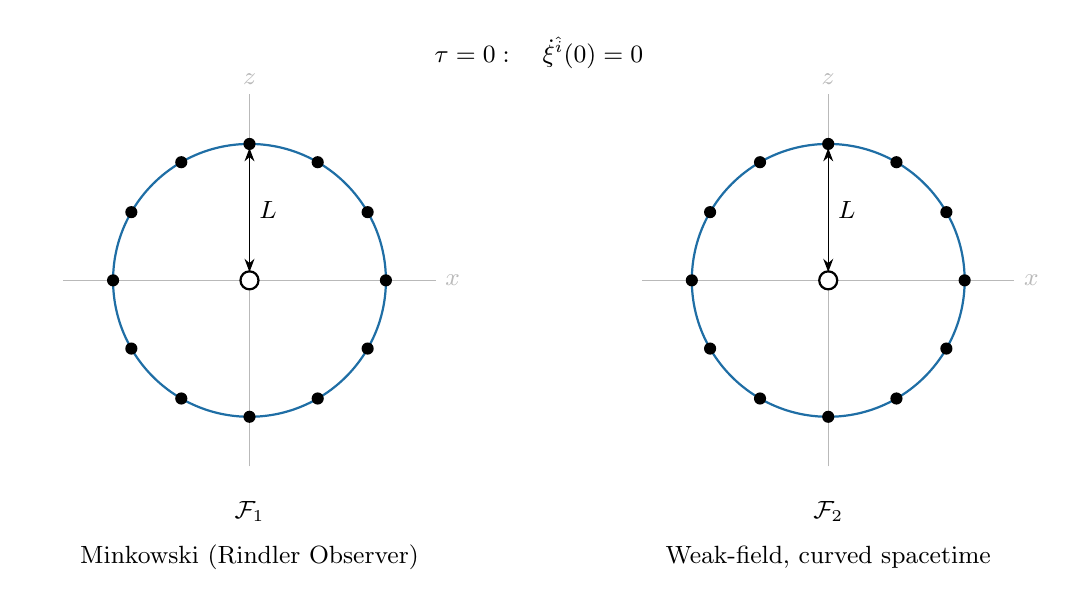
\begin{tikzpicture}[scale=1.05,font=\small]
  \foreach \shift/\frame/\desc in {0/{\mathcal F_1}/{\text{Minkowski (Rindler Observer)}},7/{\mathcal F_2}/{\text{Weak-field, curved spacetime}}} {
    \begin{scope}[shift={(\shift,0)}]
      \draw[gray!55,thin] (-2.25,0)--(2.25,0) node[right] {$x$};
      \draw[gray!55,thin] (0,-2.25)--(0,2.25) node[above] {$z$};
      \draw[flatblue,thick] (0,0) circle (1.65);
      \foreach \ang in {0,30,...,330} {\node[particle] at (\ang:1.65) {};}
      \node[centerparticle] at (0,0) {};
      \draw[<->,>=Stealth] (0,0.10)--(0,1.60) node[midway,right] {$L$};
      \node at (0,-2.8) {$\frame$};
      \node[align=center,text width=5.4cm] at (0,-3.35) {\desc};
    \end{scope}
  }
  \node at (3.5,2.75) {$\tau=0:\quad \dot\xi^{\hat i}(0)=0$};
\end{tikzpicture}
\caption{Both configurations have the same initial proper radius $L$ and zero initial relative velocity in their respective local freely falling frames. The depiction uses a vertical $xz$ plane.}
\end{figure}

In the first experiment the comoving observer will observe a static ring configuration. The geodesic deviation vanishes since there are no tidal accelerations. There are no tidal accelerations since the Riemann curvature vanishes. These statements are all downstream from the fact that the comoving observer and the freely falling test particles are moving in flat Minkowski spacetime, uniformly accelerated under hyperbolic motion. \

In the case of curved spacetime, however, \eqref{geodesic-eq-LIF} yields nonvanishing tidal accelerations. The test-particle ring will experience tidal deformation. In accordance with the hessian \eqref{tidal-acc-hessian} we see that the ring configuration will contract in the transverse directions, along the x and y axis; the ring will bulge in the radial direction along the z axis. This tidal deformation will manifest in deformation of the proper distance between the tests particles. 

\begin{figure}[h!]
\centering
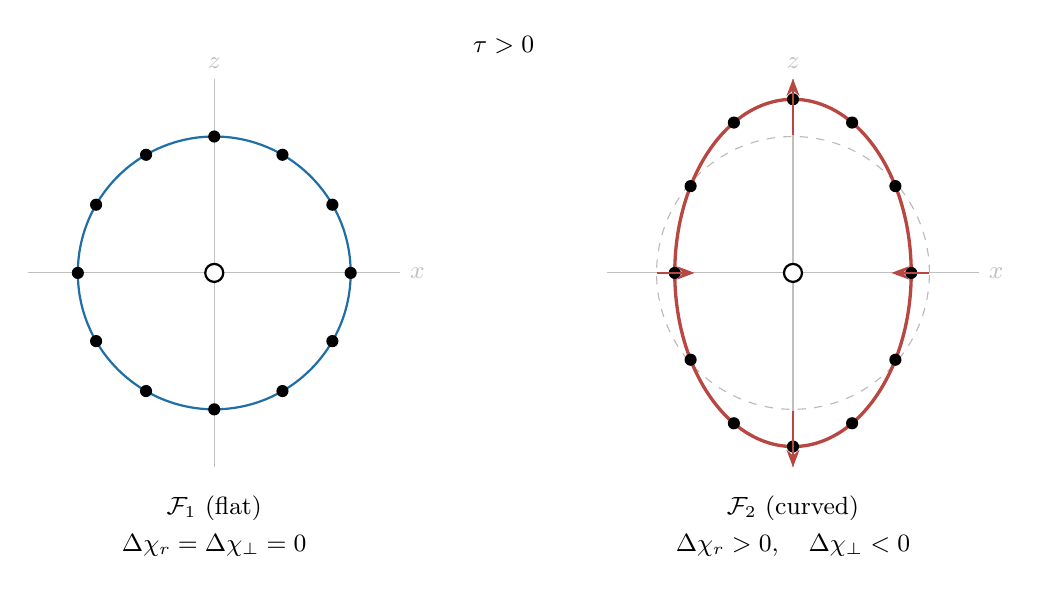
\begin{tikzpicture}[scale=1.05,font=\small]
  \def\rad{1.65}
  \def\radial{2.10}
  \def\transverse{1.43}
  \begin{scope}[shift={(0,0)}]
    \draw[gray!50,thin] (-2.25,0)--(2.25,0) node[right] {$x$};
    \draw[gray!50,thin] (0,-2.35)--(0,2.35) node[above] {$z$};
    \draw[flatblue,thick] (0,0) circle (\rad);
    \foreach \ang in {0,30,...,330} {\node[particle] at (\ang:\rad) {};}
    \node[centerparticle] at (0,0) {};
    \node at (0,-2.85) {$\mathcal F_1$ (flat)};
    \node at (0,-3.3) {$\Delta \chi_r=\Delta \chi_\perp=0$};
  \end{scope}
  \begin{scope}[shift={(7,0)}]
    \draw[gray!50,thin] (-2.25,0)--(2.25,0) node[right] {$x$};
    \draw[gray!50,thin] (0,-2.35)--(0,2.35) node[above] {$z$};
    \draw[dashed,gray!55] (0,0) circle (\rad);
    \draw[curvedred,very thick] (0,0) ellipse ({\transverse} and {\radial});
    \foreach \ang in {0,30,...,330} {
      \node[particle] at ({\transverse*cos(\ang)},{\radial*sin(\ang)}) {};
    }
    \node[centerparticle] at (0,0) {};
    \draw[fieldarrow,curvedred] (0,1.67)--(0,2.35);
    \draw[fieldarrow,curvedred] (0,-1.67)--(0,-2.35);
    \draw[fieldarrow,curvedred] (1.65,0)--(1.19,0);
    \draw[fieldarrow,curvedred] (-1.65,0)--(-1.19,0);
    \node at (0,-2.85) {$\mathcal F_2$ (curved)};
    \node at (0,-3.3) {$\Delta \chi_r>0,\quad\Delta \chi_\perp<0$};
  \end{scope}
  \node at (3.5,2.75) {$\tau>0$};
\end{tikzpicture}
\caption{Exaggerated tidal deformation of initially comoving freely falling test particles. The dashed circle is the initial configuration. To leading order near Earth, $\Delta \chi_r\simeq(gL/R_\oplus)\tau^2$ and $\Delta \chi_\perp\simeq -(gL/2R_\oplus)\tau^2$. The flat case is represented in a common local inertial frame, even if Rindler coordinates are used to describe it.}
\end{figure}

We can approximate the actual deformation by considering short observattions. For short times the equation of geodesic deviation, \eqref{geodesic-eq-LIF}, can be approximated as

\begin{equation}
    \chi^i(\tau) \approx \chi^i(0) - \frac{1}{2} R^{\hat{i}}_{\hat{\tau} \hat{j} \hat{\tau}} \chi^j(0) \tau^2
\end{equation}

Here $\tau$ is the proper time as measured by the comoving observer and $\xi(0)$ is the initial separation vector. In our test case $\chi(0) = L$ and the Riemann curvature is given by \eqref{tidal-acc-hessian}. We have two cases, one in the radial (z-axis) direction (tidal bulge); and one case in the transverse directions (x and y). Thus:

\begin{equation}
    \label{radial-separation-vector-result}
    \Delta \chi_r \approx \frac{gL}{R} \tau^2
\end{equation}

is the change in the radial direction of the proper time. And in the transverse direction

\begin{equation}
    \label{perp-separation-vector-result}
    \Delta \chi_{\perp} \approx -\frac{gL}{2R} \tau^2.
\end{equation}

The separation vectors, \eqref{radial-separation-vector-result} and \eqref{perp-separation-vector-result}, is the physical distance change the comoving observer will measure. It is worthwhile considering the order of magnitude of these tidal distortions. Consider the weak gravitational field of the Earth, such that $R=R_{\oplus}$, and a test-mass ring configuration of radius $L = 1$ m. In the comoving frame the proper time, $\tau$, is the time measured  by the comoving observer. Say the observation is taken 1 s after the beginning of the free fall. The radial tidal deformation, \eqref{radial-separation-vector-result}, is thus

\begin{equation}
    \label{estimate-radial-proper-distance}
    \Delta \chi_r = \frac{gL}{R} \tau^2 \approx \frac{(9.81\,\frac{\mathrm{m}}{\mathrm{s}^2}) (1\,\mathrm{m})}{6.371 \times 10^6\,\mathrm{m}} (1\,\mathrm{s})^2 \approx 1.54 \times 10^{-6}\,\mathrm{m}
\end{equation}

On the order of micrometers. While small, this variation in proper distances is well within the range of technology capable of measuring said variations. For instance, the LIGO detector has achieved sensitivities on the order of $10^{-18}$ m. LIGO however requires interferometers with a length of 4 km, however. In order to measure a proper distance variation on the order of \eqref{estimate-radial-proper-distance} you would require a strain sensitivity with the same order of magnitude; an order of magnitude $10^{11}$ less sensitive than the LIGO strain detectors. In fact, under the above describe conditions, an optical interferometer could be used such as a Michelson laser interferometer.

\subsection{Laser Interferometry Sketch}

Let us expand on this thought-experiment for a moment. We modify the physical configuration of our test particle and observer free fall experiment. The test particles are now fitted with a reflector which is directed at the freely falling observer at the origin of the ring. The observer will carry the basic instruments to conduct a Michelson interferometer test: a laser, beamsplitter, photodector, and a clock. We consider two test particles fittted with mirrors: $M_r$ which is fitted to the test particle aligned with the radial arm $L_r$, and $M_\perp$ fitted to the test particle aligned with the transverse arm $L_\perp$. The experiment functions as a standard Michelson interferometry experiment: a laser of some initial intensity is split by a beam splitte and directed at $M_r$ and $M_\perp$. The light is reflected by the test particles and then passed through to the photodector where the waves a combined. In practice a difference in physical distance $\Delta L$ between the radial and transverse separations will manifest as a detectable phase change $\delta \phi$.

\begin{figure}[h!]
\centering
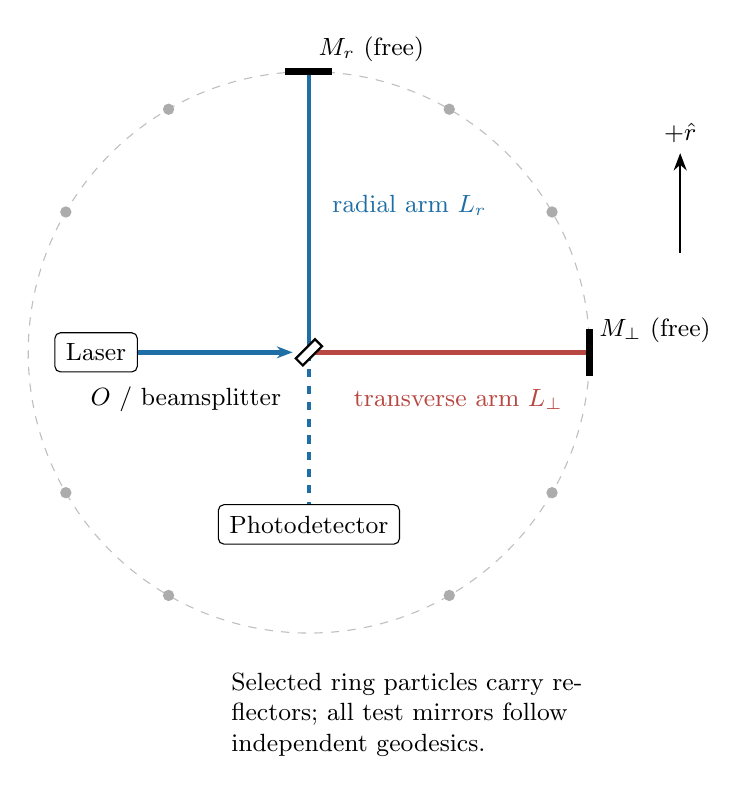
\begin{tikzpicture}[scale=1.15,font=\small]
  \coordinate (BS) at (0,0);
  \coordinate (R) at (0,3.1);
  \coordinate (H) at (3.1,0);
  \coordinate (SRC) at (-2.35,0);
  \coordinate (DET) at (0,-1.9);
  % Additional test particles on initial ring (schematic)
  \draw[gray!50,dashed] (BS) circle (3.1);
  \foreach \ang in {30,60,120,150,210,240,300,330} {
    \node[circle,fill=gray!65,inner sep=1.45pt] at (\ang:3.1) {};
  }
  % Optical paths / input-output
  \draw[laserbeam,-{Stealth[length=2mm]}] (SRC)--(-.18,0);
  \draw[laserbeam] (BS)--(R);
  \draw[armbeam] (BS)--(H);
  \draw[laserbeam,dashed,-{Stealth[length=2mm]}] (BS)--(DET);
  % central beamsplitter and mirrors
  \draw[fill=white,draw=black,thick,rotate around={45:(BS)}] (-.15,-.055) rectangle (.15,.055);
  \draw[mirror] (-.26,3.1)--(.26,3.1);
  \draw[mirror] (3.1,-.26)--(3.1,.26);
  \node[draw,fill=white,rounded corners=2pt,inner sep=4pt] at (SRC) {Laser};
  \node[draw,fill=white,rounded corners=2pt,inner sep=4pt] at (DET) {Photodetector};
  \node[above right] at (R) {$M_r$ (free)};
  \node[above right] at (H) {$M_\perp$ (free)};
  \node[below left] at (-.20,-.27) {$O$ / beamsplitter};
  \node[right,flatblue] at (.15,1.62) {radial arm $L_r$};
  \node[below,curvedred] at (1.65,-.30) {transverse arm $L_\perp$};
  \draw[fieldarrow] (4.1,1.1)--(4.1,2.2) node[above] {$+\hat r$};
  \node[align=left,text width=4.5cm] at (1.1,-4.0) {Selected ring particles carry reflectors; all test mirrors follow independent geodesics.};
\end{tikzpicture}
\caption{Michelson interferometer in a freely falling local frame. A laser and beamsplitter co-move with the central observer $O$, while the end mirrors $M_r$ and $M_\perp$ are freely falling test masses. The remaining ring particles are shown in gray. To leading order, $\delta\phi\simeq(4\pi/\lambda)(\delta L_r-\delta L_\perp)$.}
\end{figure}

The difference between the physical distances is the difference between \eqref{radial-separation-vector-result} and \eqref{perp-separation-vector-result}. The result is

\begin{equation}
    \label{physical-diff-michelson}
    \Delta L = L + \frac{gL}{R_{\oplus}} \tau^2 - \left( L -\frac{gL}{2R_{\oplus}} \tau^2 \right) = \frac{3gL}{2R_{\oplus}}\tau^2.
\end{equation}


The difference in length is due to a tidal radial elongation and transverse contraction. 

For a Michelson arm of length $L$, the round trip distance (from the beam splitter and back) is $2L$. A displacement of $\delta L$ results in a phase difference

\begin{equation}
    \label{phase-diff-1}
    \delta \phi = 2 k \delta L
\end{equation}

where k is the wave number of light with wavelength $\lambda$

\begin{equation}
    \label{wave-number}
    k = \frac{2 \pi}{\lambda}.
\end{equation}

\eqref{phase-diff-1} can be written in terms of the wavelength of light,

\begin{equation}
    \label{phase-diff-2}
    \delta \phi = \frac{4 \pi}{\lambda} \delta L.
\end{equation}

Using the approximate difference in physical distance, \eqref{physical-diff-michelson}, we would expect a phase difference in the form of

\begin{equation}
    \delta \phi = \frac{6 \pi gL}{\lambda R_{\oplus}}\tau^2.
\end{equation}

We can consider an estimate of the effect given rough physical measurements. Consider a freely falling lab near the surface of the earth with a 633 nm helium-neon laser, $L = 1.0 \mathrm{m}$, and an experiment carried out of the course of $0.10 \mathrm{s}$. The phase difference would
    
\begin{equation}
    \label{phase-diff-est}
    \delta \phi = \frac{6 \pi (9.81 \mathrm{m}/\mathrm{s}^2)(1.0 \mathrm{m})}{\left(6.33 \times 10^{-7} \mathrm{m}\right) \left(6.371 \times 10^6 \mathrm{m}\right)}(0.10 \mathrm{s})^2 \approx 0.459.
\end{equation}

We should note that the derivation for variation in physical distance due to tidal deformations was based on small, local measurements. We would expect that this result holds for quick experiments. In a realistic application of this experimental apparatus, various controls would need to be taken into account. The thought experiment assumes freely falling test particles and comoving observers. Thus, an experimental consideration would need to take into account the construction of a Michelson interferometer, absent rigid supprts, electromagnetic forces, and other affects which could interfere with the signal.

\section{Conclusions}

The purpose of this article was to provide an explicit distinction between uniform accelerated frames and uniform gravitational fields. Section 2.1 proved that the Riemann components vanishes for all indices given the uniform metric \eqref{uniform metric}. We went on to show that this result is easily understood if one realizes that the metric can be transformed into the Minkowski metric using a coordinate transformations \eqref{hyperbolic-t-coord} and \eqref{hyperbolic-x-coord}. The observer undergoing uniform proper acceleration in flat spacetime, still exists in a flat spacetime background. The physical observations taken by this observer in their frame can be explained, by an observer at rest, in flat Minkowksi spacetime and attribute them to accelerated motion. We have shown some of the similarties between uniform acceleration and uniform gravity, such as the red shifting of light. The discussion regarding tidal accelerations, however, indicated that the non-vanishing Riemann curvature of curved spacetime, such as the weak-field static metric, does indeed manifest physically. The deformation of material configurations by tidal accelerations is a measurable phenomena. In approximating this phenomena, we suggested a seemingly plausible, if not chaotic, experiment of a freely falling Michelson interferometer. The result \eqref{phase-diff-2} for the phase difference would be a empirical result, and one that would differ between the frames. In the case of uniform acceleration, the phase difference would be vanishingly small if experimental controls were in place. This is because the freely falling test particles, in flat spacetime, due not undergo any relative motion attributed to tidal accelerations. In the case of the weak-field static metric the variation in physical distance is non-zero. In the sketched apparatus, tidal elongation along the radial axis and transverse contraction would result in the reflected light along the transverse distance travelling a \textit{shorter} distance than the light travelling the radial arm. Once the light is recombined at the photodetector a phase distance, due to these arm length variations, would be measurable by the interference pattern. 

This inquiry indicates that there is a definite local constraint on the equivalence principle. We have provided an example of a local experiment, the freely falling Michelson interferometer, that can discriminate between freely falling frames in flat spacetime and those in a weak-field potential. We could further extend this discussion to experiments conducted by the uniform accelerating observers in flat spacetime, and those at rest in a uniform weak-field. Regardless of the experimental construction, the existence of tidal accelerations due to Riemann curvature in the spacetime with gravity, means that, in principle, these acceleations are measurable. As such one could construct experiments to measure the relative motion of tests masses and discern whether they are undergoing tidal accelerations, and by deduction assert the presence of a local gravitational field. The conclusion, then, is that an accelerated coordinate system in Minkowski spacetime cannot reproduce all of the phenomena of gravity.

\end{document}